\chapter{Concept and Architecture}\label{ch:concept}

This chapter presents the core contribution of the thesis: an axis library framework that decomposes
cache-aware search algorithms into interchangeable, orthogonal building-block axes, the layered
engine architecture that realizes it, the ABI-stable module interface, the nineteen-axis permutation
matrix, the probe PRT-ART, and the builder that orchestrates the three-stage evaluation. The guiding
thread is the separability problem of Section~\ref{sec:problem}: only the modular interchangeability
of the axes makes the weighting contribution of each individual constituent individually measurable
--- demonstrated empirically in Section~\ref{sec:sensitivity} and grounded methodically in
Chapter~\ref{ch:methodology}.

\section{The Axis Library Framework}\label{sec:axis-framework}

The central idea is to treat an algorithm not as a monolith but as a
\emph{composition of orthogonal axes}, each axis representing one sub-decision of a cache-aware
index (how pages are laid out, how nodes branch, how memory is allocated, how concurrency is
handled, and so on). A concrete algorithm is then a point in the Cartesian product of all axes, and
a state-of-the-art design is reconstructed as one explicit configuration. The decisive property is
\emph{modular interchangeability}: a researcher can study one new axis variant in isolation --- and
measure its effect, per axis and for the whole algorithm --- without re-implementing all the others.
This turns the comparison of two \texttt{std::map} implementations
(Section~\ref{sec:stdmap-interface}) into a controlled, reproducible experiment.

This decomposition rests on two observations. First, search algorithms share, in the large, the same
\emph{tree anatomy} in different expressions --- from balanced search trees through tries and radix
trees to custom constructs; even a sorted key--value list is, strictly speaking, a single leaf of a
tree whose values point onward to data leaves. The tree structure is therefore universal across
search-algorithm architectures and forms the canvas on which the axes are placed. Non-tree-like
search methods --- e.g.\ a hash table --- fit into the same axis system by assigning the
tree-specific axes (path compression, node type, range index) pass-through variants and carrying
only the shared axis subset; they remain the same genus with a restricted profile. A separate genus
would arise only if its base axis set differed fundamentally. Second, an instructive metaphor treats
a concrete algorithm as an \emph{organism} whose \emph{organs} are the axes: every algorithm has a
node-layout organ, a traversal organ, an allocation organ, and so on, each organ in a different
expression. Permuting the axes then resembles a genetic experiment --- exchanging organs between
organisms yields new composite algorithms with previously unknown cache-line behaviour. The research
goal is to find this shared anatomy and, within the resulting design
space (cf.\ Section~\ref{ssec:sota-design-space}), the fastest composite for a given
data-type-specific load pattern. It is precisely this modular interchangeability that solves the
separability problem of the task: because each axis can be swapped against its alternatives in
isolation while all other axes stay fixed, the weighting contribution of every single constituent to
the overall performance becomes individually measurable.

\section{Dialectical Appropriation of the State of the Art}\label{sec:dialectic}

As announced at the end of Section~\ref{sec:gap}, this thesis appropriates the inventory catalogued
in Chapter~\ref{ch:sota} \emph{dialectically} (thesis--antithesis--synthesis): per axis, a foreign
organ is \emph{adopted} or an obsolete assumption \emph{replaced}, from which the thesis's own
contribution emerges as synthesis. The guiding principle is the \enquote{third way} from
Section~\ref{ssec:aware-oblivious} --- \emph{measured} locality knowledge instead of hard-wired or
ignored cache-awareness, which makes each axis explicit as an orthogonal, permutable, and
individually measurable organ. Table~\ref{tab:dialectic} summarizes this
appropriation per composition axis, grouped by the six origin clusters from
Section~\ref{ssec:sota-corpus}; the per-axis contributing sources are listed in
Section~\ref{sec:sota-axes} (Table~\ref{tab:axes-overview}), the full building-block catalogue in
Appendix~\ref{app:blocks}.

For many axes the \emph{antithesis} is not an obsolete foreign instance but the implicit assumption
of not treating the decision as selectable at all; the synthesis then consists in making it an
explicit, measurable axis in the first place (marked \enquote{---} in the replace column). Two
cluster assignments are deliberate approximations: the cache-traversal axis~(T1) draws its impulses
from both layout theory and prefetching, and the reclamation sub-axis of the allocator~(T6) shares
its sources with synchronization~(T8) --- an inter-organ wiring, not a cluster violation.

{\footnotesize
\begin{longtable}{@{}p{2.3cm}p{3.7cm}p{2.7cm}p{3.6cm}@{}}
\caption{Dialectical appropriation of the state-of-the-art instances per composition axis}\label{tab:dialectic}\\
\toprule
\textbf{Axis} & \textbf{adopted (thesis)} & \textbf{replaced (antithesis)} & \textbf{synthesis core} \\
\midrule
\endfirsthead
\toprule
\textbf{Axis} & \textbf{adopted} & \textbf{replaced} & \textbf{synthesis core} \\
\midrule
\endhead
\bottomrule
\endlastfoot
\multicolumn{4}{@{}l}{\emph{Cluster A --- trie / node family}} \\
T0 search-algorithm & ART, HOT, START, SuRF, Wormhole; k-ary/interpolation search & monolith \enquote{structure is method} & search paradigm as permutable axis \\
T3 path-compression & byte-wise (ART), Patricia (HOT), macro-node (CoCo), multi-byte (START) & uncompressed raw path & compression granularity selectable \\
T4 node-type & ART Node4/16/48/256 & fixed node size & adaptive node class + storage delegation \\
\addlinespace
\multicolumn{4}{@{}l}{\emph{Cluster B --- hybrid / B\textsuperscript{+} / layout theory}} \\
T1 cache-traversal & cache-line stride (Chen), cache-oblivious (Bender), HBM (Schmidt) & implicit textbook linear search & algorithm and cache view separated \\
T2 mapping & linear 1:1 mapping; hash redirect, permutation index & --- & direct vs.\ pool-relative mapping explicit \\
T5 memory-layout & AoS-aligned, SoA, LOUDS bit-packed, CSS/CSB\textsuperscript{+}, AoSoA & --- & four layout dimensions permutable \\
T13 index-organization & clustered, IOT, non-clustered, heap & --- & storage order as its own axis \\
\addlinespace
\multicolumn{4}{@{}l}{\emph{Cluster C --- allocation}} \\
T6 allocator & A01--A23 (Hoard, mimalloc, jemalloc, TCMalloc, \ldots) + RCU/hazard & algorithm-hard-wired allocator & allocation as shared interface organ (seven sub-families) \\
\addlinespace
\multicolumn{4}{@{}l}{\emph{Cluster D --- prefetching}} \\
T7 prefetch & distance-estimator (ART), hardware (Wormhole), stride (Chen), adaptive & prefetch not isolated as an axis & path-oriented bundle prefetch (own) \\
\addlinespace
\multicolumn{4}{@{}l}{\emph{Cluster E --- synchronization}} \\
T8 concurrency & OLC (ART), RCU, hazard pointer; lock-/wait-free & coarse locking as the only assumption & pattern $\perp$ reclamation as two sub-axes \\
\addlinespace
\multicolumn{4}{@{}l}{\emph{Cluster F --- hardware, measurement, and engineering (TU-Dresden-adjacent)}} \\
T9 serialization & raw-binary, varint (ART), succinct (LOUDS/FST), LZ77 & --- & encoding/compression selectable \\
T10 telemetry & density tracker, insert counter, HdrHistogram, path counter & all-node counters (cache-line ping-pong) & coherence-friendly leaf-only telemetry \\
T11 value-handle & inline, external pool, immutable-shared (RCU), versioned & implicitly hard-embedded value & placement, ownership, versioning (+ chain-ref) \\
T12 ISA & vendor spec x86-64/AArch64/Power/RISC-V (+ SIMD) & --- & target ISA as compile-time axis \\
T14 I/O-dispatch & buffered, mmap, direct-IO & mmap as anti-pattern & persistence decoupled from search structure \\
T15 migration & hot/cold, multi-tier NVM, LeCaR-ML & tiering never combined with search axes & migration logic as measurable axis \\
T16 filter & Bloom, Cuckoo, SuRF range, Xor & filter never integrated with search axes & filter as orthogonal organ \\
T17 queuing-q1 & disruptor ring, delta-chain, CoW, epoch-RCU, SPSC/MPMC & operation buffer never as an axis & buffer with access-pattern classes \\
T18 queuing-q2 & eager/lazy, watermark (LSM), timed & flush policy implicit & adaptive EWMA flush policy (own) \\
\end{longtable}
}

\section{Four-Subsystem Separation (M Model)}\label{sec:m-model}

The diploma project, the cache-engine builder, the cache engine, and the probe are
\emph{four formally separated subsystems} with distinct responsibilities. The separation is
orthogonal to the three-repository split (Section~\ref{sec:repos}): builder and engine live in the
same repository but are an executable and a library, respectively.

\begin{enumerate}
  \item \textbf{\texttt{messung\_driver}} (Diplomarbeit/Code) --- the evaluation orchestrator (outer
  loop): reads the permutation-space and measurement-series XML configuration, runs the builder
  pipeline per mandatory series A/B/C, and collects the results for the appendix.
  \item \textbf{CacheEngineBuilder} (\texttt{cache-engine/apps}) --- an autonomous platform-probing
  system running, via the \texttt{ExperimentDriver} library, the seven-phase pipeline (enumerate,
  codegen, compile, load, execute, measure, persist) --- plus two opt-in phases (hot-compile of
  missing modules, ABI-contract functional test) --- and enumerating the permutation space per
  registered engine.
  \item \textbf{CacheEngine} (\texttt{cache-engine/libs}) --- the tool library: it provides, for
  each of the nineteen building-block axes (Section~\ref{sec:axes}), the default implementations and
  the associated cache-strategy families as a C++23 concept API, from which the builder assembles
  the permutation configurations.
  \item \textbf{Probe (PRT-ART)} (\texttt{prt-art}) --- an algorithm implementation registered with
  the cache engine as an \texttt{IExecutionEngine}; it supplies its own axis organs and consumes
  cache-engine services during its own lookup/insert/scan operations.
\end{enumerate}

The defining property of the M model is the \emph{bidirectional}
cache-engine~$\leftrightarrow$~probe relationship: (a) the cache engine instantiates the probe per
permutation configuration (phase 5, \textsc{execute}: \texttt{create\_instance}), and (b) the probe
calls cache-engine services (telemetry, prefetch, heuristics) during its own lookups at run time
(also phase 5, \texttt{run\_workload}); aggregation happens in phase 6 (\textsc{measure}). This
symmetry enables the \emph{multi-probe} capability: measurement series~A compares PRT-ART against
many SOTA adapters in a single builder pipeline (Figure~\ref{fig:m-model}).

\begin{figure}[!htbp]
  \centering
  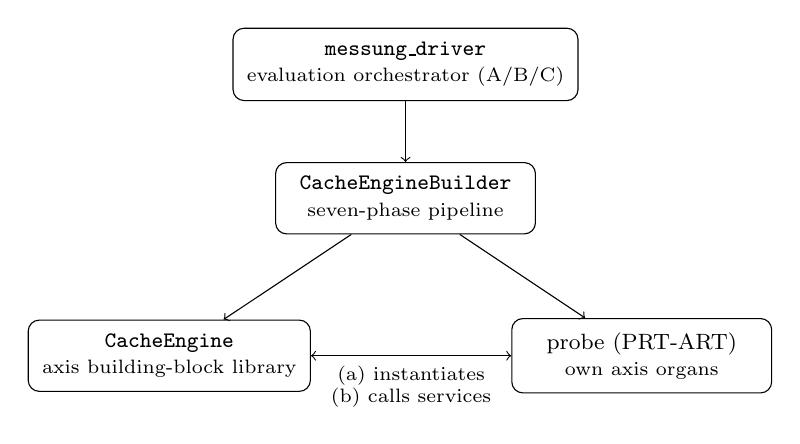
\begin{tikzpicture}[comp/.style={draw, rounded corners, align=center, font=\footnotesize, inner sep=5pt, minimum width=3.3cm}]
    \node[comp] (driver) at (0,0) {\texttt{messung\_driver}\\{\scriptsize evaluation orchestrator (A/B/C)}};
    \node[comp] (builder) at (0,-1.7) {\texttt{CacheEngineBuilder}\\{\scriptsize seven-phase pipeline}};
    \node[comp] (engine) at (-3.0,-3.7) {\texttt{CacheEngine}\\{\scriptsize axis building-block library}};
    \node[comp] (probe) at (3.0,-3.7) {probe (PRT-ART)\\{\scriptsize own axis organs}};
    \draw[->] (driver) -- (builder);
    \draw[->] (builder) -- (engine);
    \draw[->] (builder) -- (probe);
    \draw[<->] (engine) -- node[below, font=\scriptsize, align=center] {(a)~instantiates\\(b)~calls services} (probe);
  \end{tikzpicture}
  \caption{The M model: four formally separated subsystems; the \texttt{ExecutionEngine} is the
  common measurable root (not a fifth subsystem). The bidirectional
  cache-engine\,$\leftrightarrow$\,probe relationship carries the multi-probe capability.}\label{fig:m-model}
\end{figure}

Here the \texttt{ExecutionEngine} is not a fifth subsystem but the common measurable root --- the
\texttt{IExecutionEngine} interface through which these four subsystems are connected: the cache
engine provides the axis building-block library, while the ExecutionEngine contributes the
orthogonal execution and measurement infrastructure --- as the abstract root over everything
measurable (Section~\ref{sec:three-layer}), under which the probe and every engine register as an
\texttt{IExecutionEngine}.

\section{The One Architecture}\label{sec:three-layer}

The model has \emph{one} architecture --- a single, self-contained hierarchy with no parallel trees.
At its root stands the \texttt{ExecutionEngine} as the common, measurable abstraction over
everything measurable; beneath it branch the anatomy-bearing \emph{genera} --- the \texttt{SearchAlgorithm}
(the focal \emph{living organism}), the keyless \texttt{Container}, and the \texttt{Graph} with its own,
different organ set --- as well as axis-less \emph{viruses}, as siblings of the
same root (Figure~\ref{fig:one-architecture}).

\begin{figure}[!htbp]
  \centering
  \resizebox{0.92\textwidth}{!}{%
  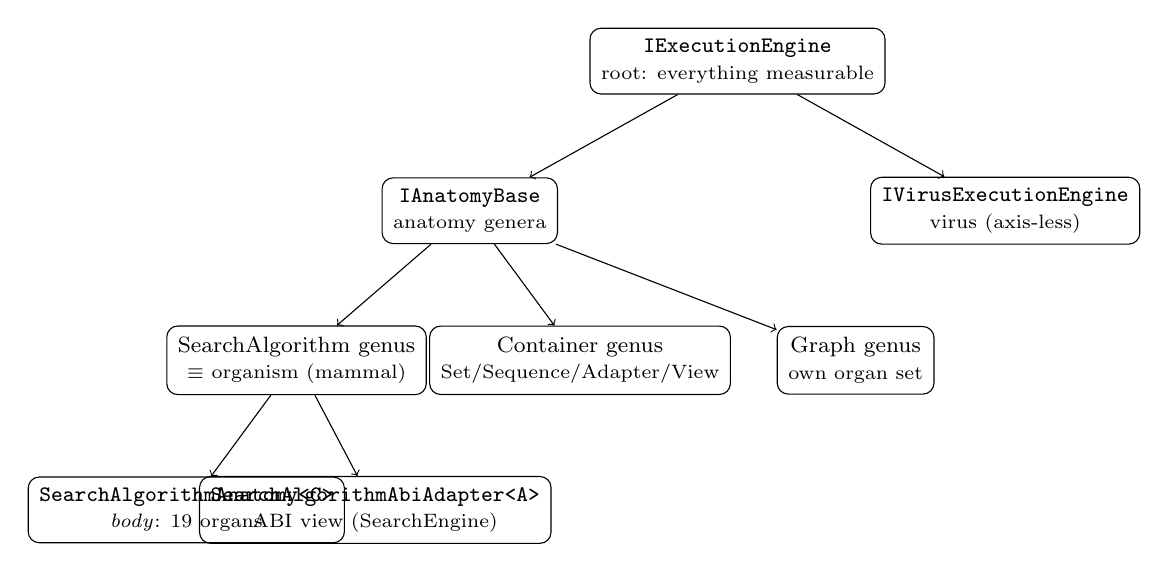
\begin{tikzpicture}[box/.style={draw, rounded corners, align=center, font=\footnotesize, inner sep=4pt}]
    \node[box] (root) at (0,0) {\texttt{IExecutionEngine}\\{\scriptsize root: everything measurable}};
    \node[box] (ana) at (-3.4,-1.9) {\texttt{IAnatomyBase}\\{\scriptsize anatomy genera}};
    \node[box] (vir) at (3.4,-1.9) {\texttt{IVirusExecutionEngine}\\{\scriptsize virus (axis-less)}};
    \node[box] (sa) at (-5.6,-3.8) {SearchAlgorithm genus\\{\scriptsize $\equiv$ \enquote{organism} (mammal)}};
    \node[box] (cont) at (-2.0,-3.8) {Container genus\\{\scriptsize Set/Sequence/Adapter/View}};
    \node[box] (graph) at (1.5,-3.8) {Graph genus\\{\scriptsize own organ set}};
    \node[box] (body) at (-7.0,-5.7) {\texttt{SearchAlgorithmAnatomy<C>}\\{\scriptsize \emph{body}: 19 organs}};
    \node[box] (abi) at (-4.6,-5.7) {\texttt{SearchAlgorithmAbiAdapter<A>}\\{\scriptsize ABI view (\enquote{SearchEngine})}};
    \draw[->] (root) -- (ana);
    \draw[->] (root) -- (vir);
    \draw[->] (ana) -- (sa);
    \draw[->] (ana) -- (cont);
    \draw[->] (ana) -- (graph);
    \draw[->] (sa) -- (body);
    \draw[->] (sa) -- (abi);
  \end{tikzpicture}}
  \caption{The \emph{one} architecture as a single hierarchy with no parallel trees: beneath the root
  branch the anatomy-bearing \emph{genera} (SearchAlgorithm, Container, Graph) and the axis-less
  \emph{viruses}. \texttt{SearchAlgorithm} \emph{is} the focal organism (mammal), its anatomy is its
  \emph{body}, and \enquote{SearchEngine} is only its ABI runtime view; Container (keyless storage)
  and Graph carry their own organ sets.}\label{fig:one-architecture}
\end{figure}

In this model a search algorithm is a \emph{living organism}, and ``organism'' and
\texttt{SearchAlgorithm} denote the same thing --- metaphor and technical term are two names for
one entity. The organism is addressed from outside through its genus interface (the test dock, a
\texttt{std::map}-like interface); its interior is its \emph{anatomy}. The anatomy is not a second
model beside the search algorithm but its \emph{body}: the fixed composition of its nineteen axes,
each corresponding to an organ. Across the module boundary the same organism is exposed as an ABI
view --- the ABI/runtime layering
\texttt{CacheEngine}\,$\to$\,\texttt{ExecutionEngine}\,$\to$\,\texttt{SearchEngine} is exactly
this view of the same organism across the module boundary, not a parallel construct:
\texttt{CacheEngine} and \texttt{ExecutionEngine} have clearly separated roles here --- the
\texttt{CacheEngine} is the \emph{axis building-block library} and provides the default axis
building blocks, whereas the \texttt{ExecutionEngine} supplies the
\emph{execution and measurement tools}: the OS primitives (cache-line-aligned allocate,
NUMA-conforming read-pin, coherence-aware write) and, in experiment mode, the measurement
aggregator over exactly one observer interface. ``SearchEngine'' is the search-API view of the
same organism, measured through exactly this one observer interface over all nineteen organs.
There is thus a single chain --- root (\texttt{ExecutionEngine}) through the genus test dock down
to the organism, which is the same thing as \texttt{SearchAlgorithm} and whose body is the anatomy
with its nineteen axes.

\subsection{Three Levels and the Wiring of the Organs}\label{ssec:three-levels}

Within this one hierarchy three levels can be distinguished. The topmost is the \emph{genus} --- the
externally visible algorithm interface (the test dock): \texttt{SearchAlgorithm} (the key--value
interface and the focus of this thesis), \texttt{Container} (keyless storage), and \texttt{Graph}.
Beneath it lies the \emph{genus subclass}, which fixes an axis set: under \texttt{SearchAlgorithm}
the full nineteen-axis anatomy (in the biological reading the ``mammal''), under \texttt{Container}
the subclasses Set, Sequence, Adapter, and View (metaphorically ``bird'', ``reptile'', ``invertebrate'',
``plant''); \texttt{Graph} carries its own, different organ set. The lowest level is formed by the
\emph{organs} themselves --- for the SearchAlgorithm anatomy the nineteen axes (T0--T18) that are
permuted within this subclass.

The anatomy thus introduced is more than the mere enumeration of these organs: it is their
\emph{wiring}. Each organ exports a generalized interface through which the remaining organs draw on
its services without knowing its concrete assignment. The allocation organ, for instance, provides a
shared allocation interface that node layout, value storage, and serialization use for their memory
needs --- regardless of which concrete allocator (Section~\ref{sec:axes}) sits behind it. A known
search algorithm therefore appears in this model not as a monolithic block but as a particular
interconnection of generic organ interfaces. It is precisely this interconnection that makes it
possible to exchange a single organ --- and thereby to span the permutation space of
Section~\ref{sec:axes} --- without re-implementing the remaining organs.

\section{ABI-Stable C++23 Module Interface}\label{sec:abi}

The ABI follows the variadic-template principle: the hybrid API specializes by parameter count
(1/2/$N$, cf.\ Section~\ref{sec:stdmap-interface} and the listing in Figure~\ref{fig:abi}). Complex
keys are reduced to fixed-length
16-byte binary strings by a fingerprint component. The module boundary is binary-stable so that
the builder can load pre-compiled permutation modules (LoadLibrary/dlopen) and verify the ABI
contract per module (Figure~\ref{fig:abi}).

\begin{figure}[!htbp]
\begin{lstlisting}[basicstyle=\footnotesize\ttfamily,frame=single,xleftmargin=1.5em]
// C-stable module boundary: exports exactly ONE organism per permutation
extern "C" IAnatomyBase* comdare_create_anatomy();

// Variadic hybrid API by parameter count (key K, values V):
//   1 parameter  ->  std::vector<V>
//   2 parameters ->  std::map<K, V>
//   N > 2        ->  std::map<K, std::tuple<V1, ..., VN>>
template<class... Ts> class SearchEngine;   // ABI runtime view of the organism
\end{lstlisting}
  \caption{The ABI-stable C module boundary and the variadic hybrid API. Complex keys are reduced to
  fixed-length 16-byte binary strings by a fingerprint component.}\label{fig:abi}
\end{figure}

\section{The Building-Block Axes}\label{sec:axes}

After the N-phase extension and the consolidation into the search-algorithm anatomy, the matrix
comprises \textbf{nineteen main axes (T0--T18) plus roughly sixty-four sub-axes} --- the seventeen
search axes (search-algorithm, cache-traversal, mapping, path-compression, node-type, memory-layout,
allocator, prefetch, concurrency, serialization, telemetry, value-handle, ISA, index-organization,
I/O-dispatch, migration, filter) plus the two queuing axes, exactly the organs that the
\texttt{IsComposition} concept enforces per algorithm. The sub-axes and the per-axis contributing
building blocks are listed in Table~\ref{tab:axes-overview} and, in detail, Appendix~\ref{app:blocks}.
Per axis a variant family (a \texttt{std::variant} in the building-block prototype) enumerates all
concretizations --- the allocator axis alone offers about two dozen ---; the Cartesian product of the
main axes spans around $10^{14}$ configurations (Section~\ref{sec:explosion}).

\section{PRT-ART as Probe}\label{sec:prt-art}

PRT-ART is a \emph{probe}: an abstract organism that supplies some axis organs itself and, for the
rest, falls back at compile time (\texttt{resolve\_baustein.hpp}) onto the cache-engine default
building blocks where it does not override an axis; the hybrid
\texttt{PrtArtSearchEngine<Ts\ldots>} API stays untouched. Its run-time binding is through the
execution-engine adapter, not through a search-engine layer of its own. PRT-ART contributes its
own implementations in the build-axis page-type as well as the layout, allocator, prefetch,
concurrency-pattern, and telemetry organs (4+2 pool allocator in the free-list sub-axis, path-oriented (bundle) prefetch, OLC with reserved value blocks, and the
H1/H2/H3 metrics); for the remaining axes it reuses existing SOTA building blocks via permutation
configuration.

\section{CacheEngineBuilder and Three-Stage Evaluation}\label{sec:builder}

The builder orchestrates a three-stage evaluation: \textbf{stage~1} (cache-engine only) uses the
default variant per axis; \textbf{stage~2} (probe only) replaces the overridden axes with the
probe variants and keeps cache-engine defaults elsewhere; \textbf{stage~3} (full join,
non-redundant) combines the default and all probe variants. Each stage can emit up to thousands of
non-redundant permutation binaries, each loaded at run time as an ABI-stable C++23 module; the present
measurement run materializes only a sparse, capped subset (Figure~\ref{fig:three-stage}).

\begin{figure}[!htbp]
  \centering
  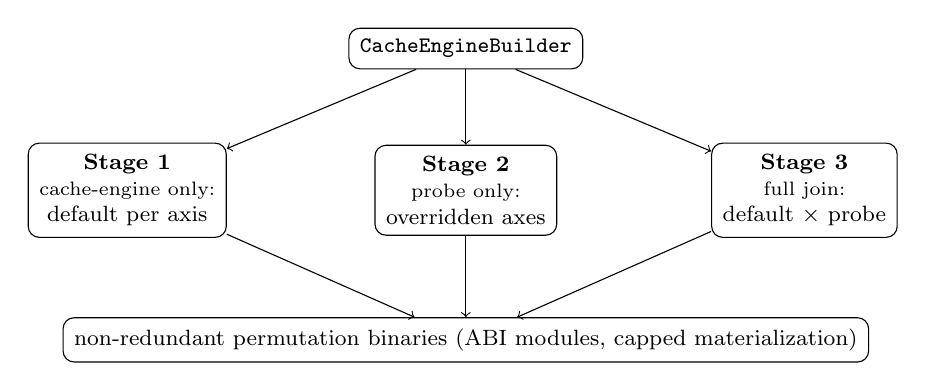
\begin{tikzpicture}[stage/.style={draw, rounded corners, align=center, font=\footnotesize, inner sep=4pt}]
    \node[draw, rounded corners, font=\footnotesize, inner sep=4pt] (b) at (0,0) {\texttt{CacheEngineBuilder}};
    \node[stage] (s1) at (-4.3,-1.8) {\textbf{Stage~1}\\\scriptsize cache-engine only:\\default per axis};
    \node[stage] (s2) at (0,-1.8) {\textbf{Stage~2}\\\scriptsize probe only:\\overridden axes};
    \node[stage] (s3) at (4.3,-1.8) {\textbf{Stage~3}\\\scriptsize full join:\\default $\times$ probe};
    \node[draw, rounded corners, align=center, font=\footnotesize, inner sep=4pt] (out) at (0,-3.7) {non-redundant permutation binaries (ABI modules, capped materialization)};
    \draw[->] (b) -- (s1);
    \draw[->] (b) -- (s2);
    \draw[->] (b) -- (s3);
    \draw[->] (s1) -- (out);
    \draw[->] (s2) -- (out);
    \draw[->] (s3) -- (out);
  \end{tikzpicture}
  \caption{The builder's three-stage evaluation: each stage emits non-redundant permutation
  binaries; their mapping to the measurement series~A/B/C is shown in
  Table~\ref{tab:stage-series}.}\label{fig:three-stage}
\end{figure}

These stages do \emph{not} map one-to-one onto the three mandatory measurement series of
Chapter~\ref{ch:methodology}; rather, they feed them as follows: the default binaries of stage~1
(cache-engine building blocks, including the reconstructed state-of-the-art profiles) and the probe
binaries of stage~2 \emph{jointly} form comparison series~A (probe versus state of the art); the
non-redundant full join of stage~3 is the basis of variation series~B (systematic permutation of the
design decisions under otherwise equal conditions). Regression series~C (merge/regression old versus
new), by contrast, is bound to no single stage but runs across builds over successive states of the
same configuration. Table~\ref{tab:stage-series} summarizes this mapping.

\begin{table}[!htbp]
  \centering
  \caption{Mapping of the three-stage evaluation to the mandatory measurement series}\label{tab:stage-series}
  \begin{tabular}{@{}lll@{}}
    \toprule
    \textbf{Evaluation stage} & \textbf{Content} & \textbf{feeds series} \\
    \midrule
    Stage~1 (cache-engine only) & default building blocks + SOTA profiles & A (baseline also for C) \\
    Stage~2 (probe only) & overridden axes = probe variants & A \\
    Stage~3 (full join) & default $\times$ probe, non-redundant & B \\
    across builds & old versus new of the same configuration & C \\
    \bottomrule
  \end{tabular}

  \smallskip
  {\footnotesize The three evaluation stages map not one-to-one but in this assignment onto the three
  mandatory measurement series~A/B/C; series~C is build-/version-spanning (not bound to a single
  test stage).\par}
\end{table}

From the
fine-grained measurement results the pipeline already provides the required ranking; the automatic
selection of the best overall algorithm and its delivery as a standalone, ABI-stable binary behind
the unified search-algorithm interface are envisioned as an extension (objective, outlook).

\subsection{Heuristic Profile Evaluation and Binary Selection}\label{sec:heuristic-profile-selection}

Beyond the bare ranking, an end-to-end evaluation step is envisioned as an \emph{objective and
outlook} that automatically turns the fine-grained measurement results into a delivered
configuration: from the ranking of the three measurement series the best axis composition is
determined per load and data-type profile, an \emph{ML classifier} predicts this configuration from
the axis and load-profile features (access distribution, write/read ratio, key/value data type), and
the result is stored as a reusable XML load profile --- symmetric to the measurement-series XML
configurations from Section~\ref{sec:m-model}. This selection and delivery mechanism is, in the
current state, \emph{not yet implemented}; its detailed treatment is given in the evaluation
methodology (Section~\ref{sec:measurements-to-heuristics}) and in the outlook (Chapter~\ref{ch:conclusion}).
